    \begin{tabular}{p{1.8cm}<{\centering}|m{3cm}<{\centering}|c|p{2.3cm}<{\centering}|c|c}
    Global category & Example diagram & Bkg rej. discriminant & Splitting method to target STXS bins & Targeted STXS bins (\# of bins) & \# of tags \\ \hline
    tHq leptonic & \vspace{.1cm}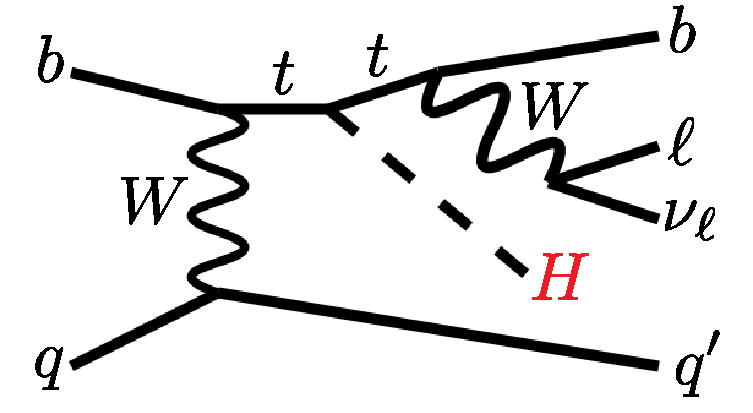
\includegraphics[width=2.5cm]{Figures/hgg_overview/categorisation_feynman/thq_lep.pdf} & \begin{tabular}{c}{tHq leptonic BDT-bkg\\top DNN (tH-vs-ttH)}\end{tabular} & None & tHq & 1 \\ \hline
    
    ttH leptonic & \vspace{.1cm}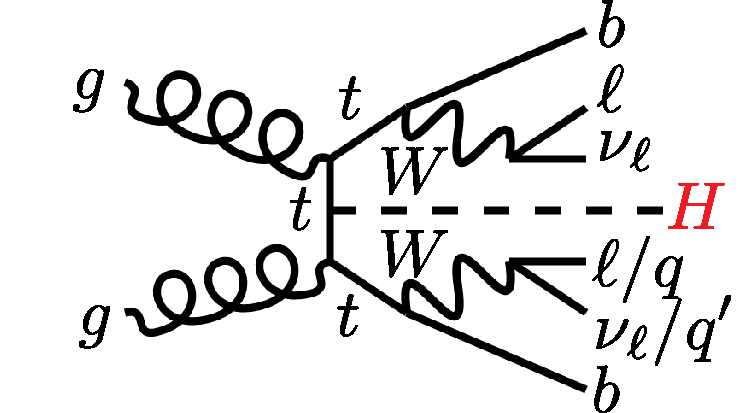
\includegraphics[width=2.5cm]{Figures/hgg_overview/categorisation_feynman/tth_lep.pdf} & \begin{tabular}{c}{ttH leptonic BDT-bkg\\top DNN (tH-vs-ttH)}\end{tabular} & Reco $p_T^{\gamma\gamma}$ & \begin{tabular}{c}{ttH~\ptH~$<$~60 \\ ttH~120~$<$~\ptH~$<$~120 \\ ttH~120~$<$~\ptH~$<$~200 \\ ttH~200~$<$~\ptH~$<$~300 \\ ttH~\ptH~$>$~300}\end{tabular} & \begin{tabular}{c}{3 \\ 3 \\ 2 \\ 1 \\ 1}\end{tabular} \\ \hline
    
    ZH leptonic & \vspace{.1cm}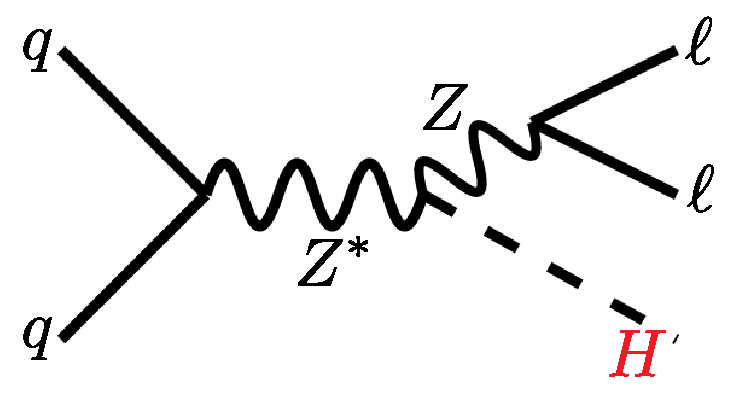
\includegraphics[width=2.5cm]{Figures/hgg_overview/categorisation_feynman/zh_lep.pdf} & ZH leptonic BDT & None & All ZH lep and ggZH lep bins (10) & 2 \\ \hline
    
    WH leptonic & \vspace{.1cm}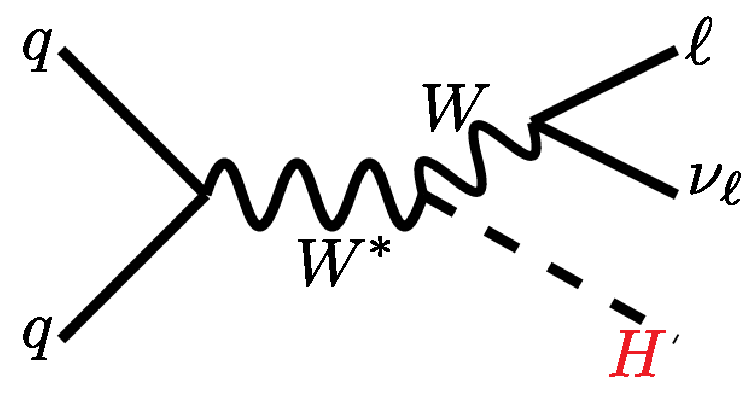
\includegraphics[width=2.5cm]{Figures/hgg_overview/categorisation_feynman/wh_lep.pdf} & WH leptonic BDT & Reco $p_T^{\gamma\gamma}$ & \begin{tabular}{c}{WH lep~$p_T^V<75$ \\ WH lep~$75<p_T^V<150$ \\ WH lep~$p_T^V>150$ (3)}\end{tabular} & \begin{tabular}{c}{2 \\ 2 \\ 1}\end{tabular} \\ \hline
    
    VH MET & \vspace{.1cm}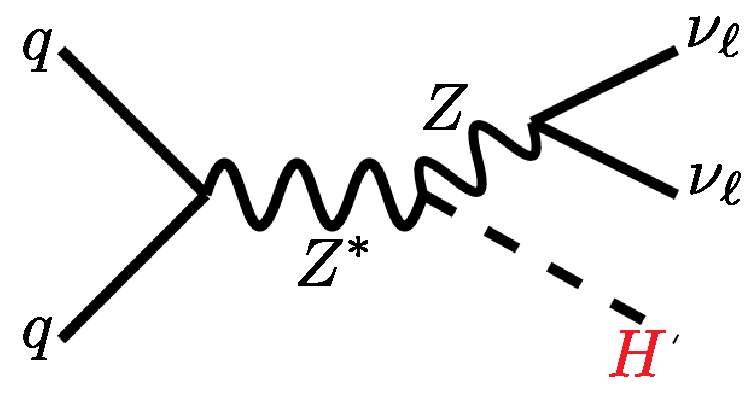
\includegraphics[width=2.5cm]{Figures/hgg_overview/categorisation_feynman/vh_met.pdf} & VH MET BDT & None & All VH lep bins (15) & 3 \\ \hline
    
    ttH hadronic & \vspace{.1cm}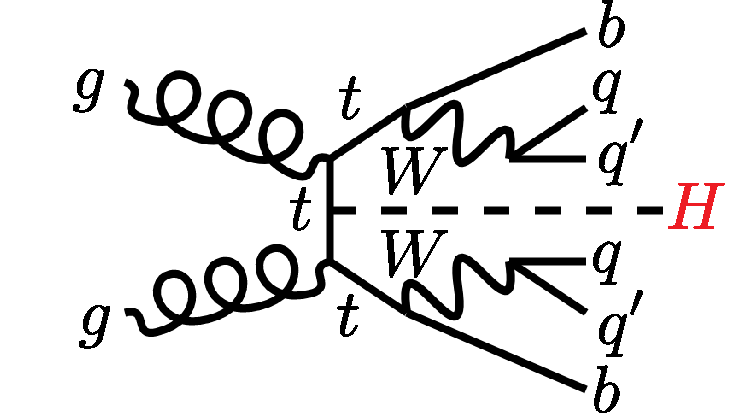
\includegraphics[width=2.5cm]{Figures/hgg_overview/categorisation_feynman/tth_had.pdf} & ttH hadronic BDT-bkg & Reco $p_T^{\gamma\gamma}$ & \begin{tabular}{c}{ttH~\ptH~$<$~60 \\ ttH~120~$<$~\ptH~$<$~120 \\ ttH~120~$<$~\ptH~$<$~200 \\ ttH~200~$<$~\ptH~$<$~300 \\ ttH~\ptH~$>$~300}\end{tabular} & \begin{tabular}{c}{3 \\ 3 \\ 4 \\ 3 \\ 2}\end{tabular} \\ \hline
    
    \multirow{2}{*}{\begin{tabular}{c}{~\\~\\~\\VBF-like}\end{tabular}} & \vspace{.1cm}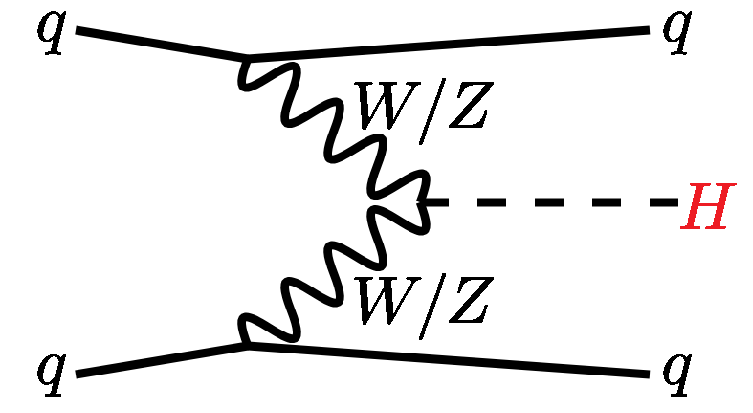
\includegraphics[width=2.5cm]{Figures/hgg_overview/categorisation_feynman/vbf.pdf} & \multirow{2}{*}{\begin{tabular}{c}{~\\~\\Dijet BDT\\Diphoton BDT}\end{tabular}} & Reco $p_T^{\gamma\gamma}$, $p_T^{\gamma\gamma jj}$, $m_{jj}$ & \begin{tabular}{c}{qqH BSM \\ qqH VBF-like low $m_{jj}$ low $p_T^{Hjj}$ \\ qqH VBF-like low $m_{jj}$ high $p_T^{Hjj}$ \\ qqH VBF-like high $m_{jj}$ low $p_T^{Hjj}$ \\ qqH VBF-like high $m_{jj}$ high $p_T^{Hjj}$ }\end{tabular} & \begin{tabular}{c}{2 \\ 2 \\ 2 \\ 2 \\ 2}\end{tabular} \\ \cline{2-2} \cline{4-6}
    & \vspace{.1cm}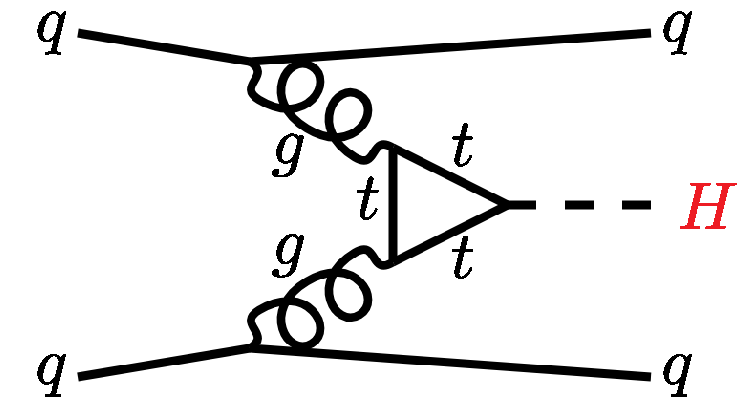
\includegraphics[width=2.5cm]{Figures/hgg_overview/categorisation_feynman/ggh_vbflike.pdf} & & None & All ggH VBF-like bins (4) & 2 \\ \hline
    
    VH hadronic & \vspace{.1cm}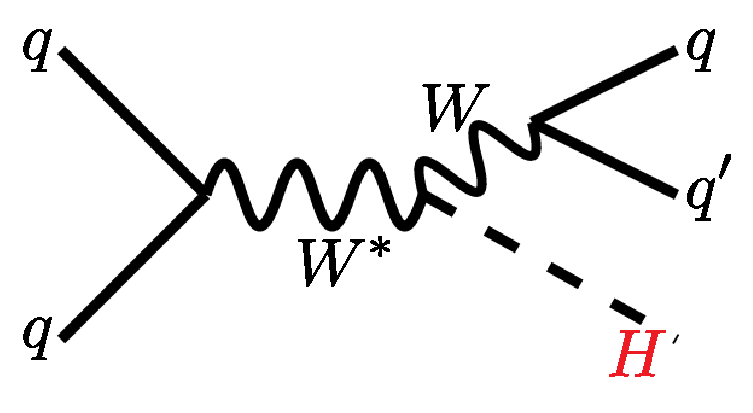
\includegraphics[width=2.5cm]{Figures/hgg_overview/categorisation_feynman/vh_had.pdf} & \begin{tabular}{c}{VH hadronic BDT\\Diphoton BDT}\end{tabular} & None & qqH VH-like & 2 \\ \hline
    
    ggH & \vspace{.1cm}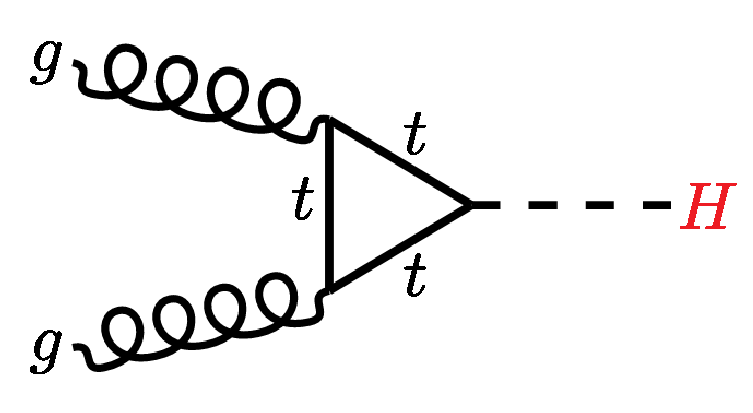
\includegraphics[width=2.5cm]{Figures/hgg_overview/categorisation_feynman/ggh.pdf} & Diphoton BDT & ggH BDT + Reco $p_T^{\gamma\gamma}$ for high \ptH region & \begin{tabular}{c}{ggH 0J low \ptH \\ ggH 0J high \ptH \\ ggH 1J low \ptH \\ ggH 1J med \ptH \\ ggH 1J high \ptH \\ ggH $\geq$2J low \ptH \\ ggH $\geq$2J med \ptH \\ ggH $\geq$2J high \ptH \\ ggH BSM $200<p_T^H<300$ \\ ggH BSM $300<p_T^H<450$ \\ ggH BSM $450<p_T^H<650$ \\ ggH BSM $p_T^H>650$}\end{tabular} & \begin{tabular}{c}{3 \\ 3 \\ 3 \\ 3 \\ 3 \\ 3 \\ 3 \\ 3 \\ 2 \\ 2 \\ 1 \\ 1}\end{tabular} \\ \hline
    
    No dedicated category & - & - & - & \begin{tabular}{c}{qqH 0J, 1J, $\geq$2J $m_{jj}<60$ \\ qqH $\geq$2J $120<m_{jj}<350$ \\ bbH, tHW}\end{tabular} & 0 \\ \hline
    
    \multicolumn{5}{r|}{Total$\quad$} & 80 \\
    \end{tabular}